\documentclass[a4paper,12pt]{article}
\usepackage[utf8]{vietnam}
\usepackage{graphicx}
\usepackage{setspace}
\usepackage{geometry}
\geometry{left=3cm,right=2cm,top=2cm,bottom=2cm}

\begin{document}

% ================= TRANG BÌA =================
\begin{center}
{\bfseries\large TRƯỜNG ĐẠI HỌC GIAO THÔNG VẬN TẢI TP. HỒ CHÍ MINH\\
VIỆN CÔNG NGHỆ THÔNG TIN VÀ ĐIỆN, ĐIỆN TỬ}\\[1cm]


\includegraphics[width=9cm]{uth_log.png}\\[1cm] % Thay hình logo tại đây

{\bfseries\Large BÁO CÁO BÀI TẬP LỚN}\\[0.4cm]
{\bfseries\large MÔN LẬP TRÌNH THIẾT BỊ DI ĐỘNG}\\[1cm]

{\bfseries Nhóm 08}\\[0.3cm]
{\bfseries Đề tài: Ứng dụng game-pixel-adventure}\\[1cm]

\begin{flushleft}
\textbf{Giảng viên:} Thầy Trương Quang Tuấn\\[0.4cm]
\textbf{Thành viên nhóm:}\\[0.3cm]

\begin{tabular}{|c|c|c|}
\hline
\textbf{MSSV} & \textbf{Họ và tên} & \textbf{Lớp} \\
\hline
070205010679 & Trần Văn Tuấn & CN23Q2D \\
070205000427 & Trần Đức Hiếu & CN23Q2D \\
\hline
\end{tabular}
\end{flushleft}

\vfill
TP Hồ Chí Minh, ngày 15 tháng 11 năm 2025

\end{center}

\newpage

% ================= MỤC LỤC =================
\begin{center}
{\bfseries\Large MỤC LỤC}
\end{center}

\tableofcontents

\newpage

% ================= LỜI MỞ ĐẦU =================
\section*{LỜI MỞ ĐẦU}
\addcontentsline{toc}{section}{LỜI MỞ ĐẦU}

Trong bối cảnh công nghệ số phát triển mạnh mẽ, các thiết bị di động ngày càng phổ biến và trở thành một phần không thể thiếu trong cuộc sống hiện đại. Cùng với đó, ngành công nghiệp trò chơi trên thiết bị di động cũng không ngừng tăng trưởng và đổi mới, mang đến cơ hội trải nghiệm giải trí phong phú cho người dùng.

Đặc biệt, các trò chơi mang phong cách Pixel Art đang dần quay trở lại và khẳng định sức hút riêng nhờ lối thiết kế đơn giản nhưng sáng tạo, phù hợp với hiệu năng và kích thước màn hình của thiết bị di động. Việc phát triển một trò chơi 2D trên nền tảng Unity không chỉ mang lại cơ hội tiếp xúc thực tiễn với quy trình tạo lập game, mà còn giúp sinh viên vận dụng hiệu quả kiến thức môn học vào sản phẩm thực tế.

Xuất phát từ những lý do đó, nhóm chúng em đã thực hiện đề tài \textbf{“Ứng dụng game Pixel-Adventure”} trong khuôn khổ môn \textbf{Lập trình thiết bị di động}. Đề tài hướng đến việc xây dựng một tựa game phiêu lưu đi cảnh (platformer) với gameplay cơ bản nhưng thú vị, tích hợp các cơ chế điều khiển thân thiện cho người dùng Android và đảm bảo hiệu suất ổn định.

Trong quá trình thực hiện, nhóm đã áp dụng kiến thức về Unity, C\# Script, thiết kế giao diện người dùng, kiểm thử và tối ưu game. Bên cạnh đó, nhóm cũng rèn luyện được kỹ năng làm việc nhóm, quản lý tiến độ và giải quyết các vấn đề phát sinh trong quá trình phát triển sản phẩm.

Mặc dù thời gian thực hiện có hạn và vẫn còn những thiếu sót, nhưng nhóm hy vọng rằng sản phẩm này thể hiện được tinh thần sáng tạo, sự cố gắng và học hỏi nghiêm túc của các thành viên. Nhóm kính mong nhận được những ý kiến đóng góp của thầy để hoàn thiện game tốt hơn trong tương lai.

\vspace{0.5cm}
\hfill \textit{Nhóm thực hiện}

\newpage

% ================= CHƯƠNG 1 =================
\section{GIỚI THIỆU ĐỀ TÀI}

\subsection{Lý do chọn đề tài}

Trong thời đại hiện nay, game mobile ngày càng phát triển và trở thành một ngành công nghiệp giải trí đầy tiềm năng. Các trò chơi đồ họa Pixel Art trở lại mạnh mẽ nhờ phong cách nghệ thuật đơn giản nhưng hấp dẫn, tối ưu cho thiết bị di động.

Vì vậy, nhóm chọn đề tài \textbf{Game Pixel-Adventure} nhằm:
\begin{itemize}
    \item Áp dụng kiến thức môn Lập trình thiết bị di động và Unity vào một dự án cụ thể.
    \item Tự tạo một sản phẩm game hoàn chỉnh có thể cài đặt và trải nghiệm trên thiết bị Android thực tế.
    \item Khám phá quy trình phát triển game từ ý tưởng $\rightarrow$ thiết kế $\rightarrow$ triển khai $\rightarrow$ kiểm thử.
\end{itemize}

\subsection{Mục tiêu xây dựng game}

Các mục tiêu chính của đề tài:
\begin{itemize}
    \item Phát triển một game nhập vai phiêu lưu 2D dạng platformer trên nền tảng Unity.
    \item Hỗ trợ điều khiển nhân vật bằng joystick ảo trên Android, phù hợp với thiết bị màn hình cảm ứng.
    \item Thiết kế hệ thống kẻ địch, cạm bẫy, vật phẩm, điểm số và điều kiện thắng/thua rõ ràng.
    \item Xây dựng gameplay mượt mà, đồ họa Pixel Art đẹp mắt, hiệu suất ổn định.
    \item Đóng gói và cài đặt game trên thiết bị Android thực tế để demo.
\end{itemize}

\subsection{Phạm vi thực hiện}

Phạm vi của đề tài được giới hạn như sau:
\begin{itemize}
    \item Game platform 2D dạng side-scrolling.
    \item Xây dựng khoảng từ 1 đến 2 màn chơi mẫu có đầy đủ: vật cản, quái, điểm thưởng.
    \item Hỗ trợ Android với API từ 21 trở lên.
    \item Không tích hợp hệ thống tài khoản, mua hàng trong game hay lưu trữ trên server.
\end{itemize}

\subsection{Ý nghĩa thực tiễn}

Đề tài mang lại một số ý nghĩa thực tiễn:
\begin{itemize}
    \item Nâng cao kỹ năng sử dụng Unity và C\# trong phát triển game.
    \item Giúp sinh viên hiểu rõ hơn về quy trình phát triển và phát hành game mobile.
    \item Tạo ra một sản phẩm thực tế có thể demo trong các buổi báo cáo, triển lãm, hoặc đưa vào portfolio cá nhân.
\end{itemize}

\newpage

% ================= CHƯƠNG 2 =================
\section{CÔNG NGHỆ SỬ DỤNG}

\subsection{Unity Engine}

Trong đề tài này, nhóm sử dụng Unity Engine phiên bản 2021 trở lên. Đây là công cụ phát triển game đa nền tảng phổ biến, hỗ trợ tốt cho game 2D và 3D.

\textbf{Một số ưu điểm của Unity:}
\begin{itemize}
    \item Giao diện trực quan, hỗ trợ kéo-thả (drag and drop).
    \item Kho tài nguyên phong phú từ Unity Asset Store.
    \item Hỗ trợ build đa nền tảng: PC, Android, iOS, WebGL, \ldots
    \item Cộng đồng lớn, tài liệu và tutorial rất nhiều.
\end{itemize}

\subsection{C\# Script trong Unity}

Unity sử dụng ngôn ngữ C\# để lập trình logic game. Trong game Pixel-Adventure, nhóm sử dụng C\# để:
\begin{itemize}
    \item Điều khiển nhân vật (di chuyển, nhảy, va chạm, thu thập vật phẩm).
    \item Xử lý hành vi kẻ địch (đi tuần, đổi hướng, bị tiêu diệt khi bị stomp, \ldots).
    \item Quản lý điểm số, thời gian, trạng thái thắng/thua.
    \item Quản lý giao diện người dùng (HUD, menu, panel Game Over/Win).
\end{itemize}

\textbf{Một số script tiêu biểu:}
\begin{itemize}
    \item \texttt{PlayerController.cs}: Xử lý di chuyển, nhảy, kiểm tra va chạm.
    \item \texttt{EnemyController.cs}: Xử lý hành vi kẻ địch, vùng di chuyển patrol.
    \item \texttt{ItemPickup.cs}: Xử lý thu thập vật phẩm, tăng điểm.
    \item \texttt{GameManager.cs}: Quản lý trạng thái game (pause, game over, win).
\end{itemize}

\subsection{Pixel Art cho đồ họa 2D}

Game sử dụng phong cách Pixel Art với các sprite kích thước 16$\times$16 hoặc 32$\times$32, giúp:
\begin{itemize}
    \item Tối ưu hiệu năng cho GPU trên thiết bị di động.
    \item Tạo phong cách đồ họa retro, đơn giản nhưng cuốn hút.
\end{itemize}

Các nguồn Sprite có thể đến từ:
\begin{itemize}
    \item Tự thiết kế bằng Aseprite, Photoshop, \ldots
    \item Tài nguyên miễn phí trên Unity Asset Store hoặc các nguồn open-source.
\end{itemize}

\subsection{Build game trên Android}

Để build game lên Android, nhóm thực hiện:
\begin{itemize}
    \item Cài đặt Android Build Support cùng với SDK/NDK trong Unity Hub.
    \item Cấu hình Player Settings: tên package, icon, orientation màn hình, \ldots
    \item Thiết lập hệ thống điều khiển bằng các nút UI (joystick, nút nhảy).
    \item Xuất bản dưới dạng file \texttt{.apk} hoặc \texttt{.aab}.
\end{itemize}

\newpage

% ================= CHƯƠNG 3 =================
\section{PHÂN TÍCH VÀ THIẾT KẾ}

\subsection{Phân tích yêu cầu}

\begin{center}
\begin{tabular}{|p{4cm}|p{9cm}|}
\hline
\textbf{Nhóm yêu cầu} & \textbf{Mô tả} \\
\hline
Gameplay & Nhân vật phiêu lưu, né cạm bẫy, tiêu diệt kẻ địch, thu thập vật phẩm. \\
\hline
Điều khiển & Joystick ảo cho di chuyển trái/phải, nút nhảy riêng, hỗ trợ mobile. \\
\hline
Tương tác & Va chạm vật phẩm để tăng điểm, va chạm trap hoặc enemy không đúng cách sẽ Game Over. \\
\hline
Hiệu suất & Đảm bảo FPS ổn định $\geq$ 30 trên Android trong suốt quá trình chơi. \\
\hline
Đồ họa & Phong cách Pixel Art 2D side-scrolling. \\
\hline
\end{tabular}
\end{center}

\subsection{Sơ đồ Use Case (mô tả)}

Các Use Case chính:
\begin{itemize}
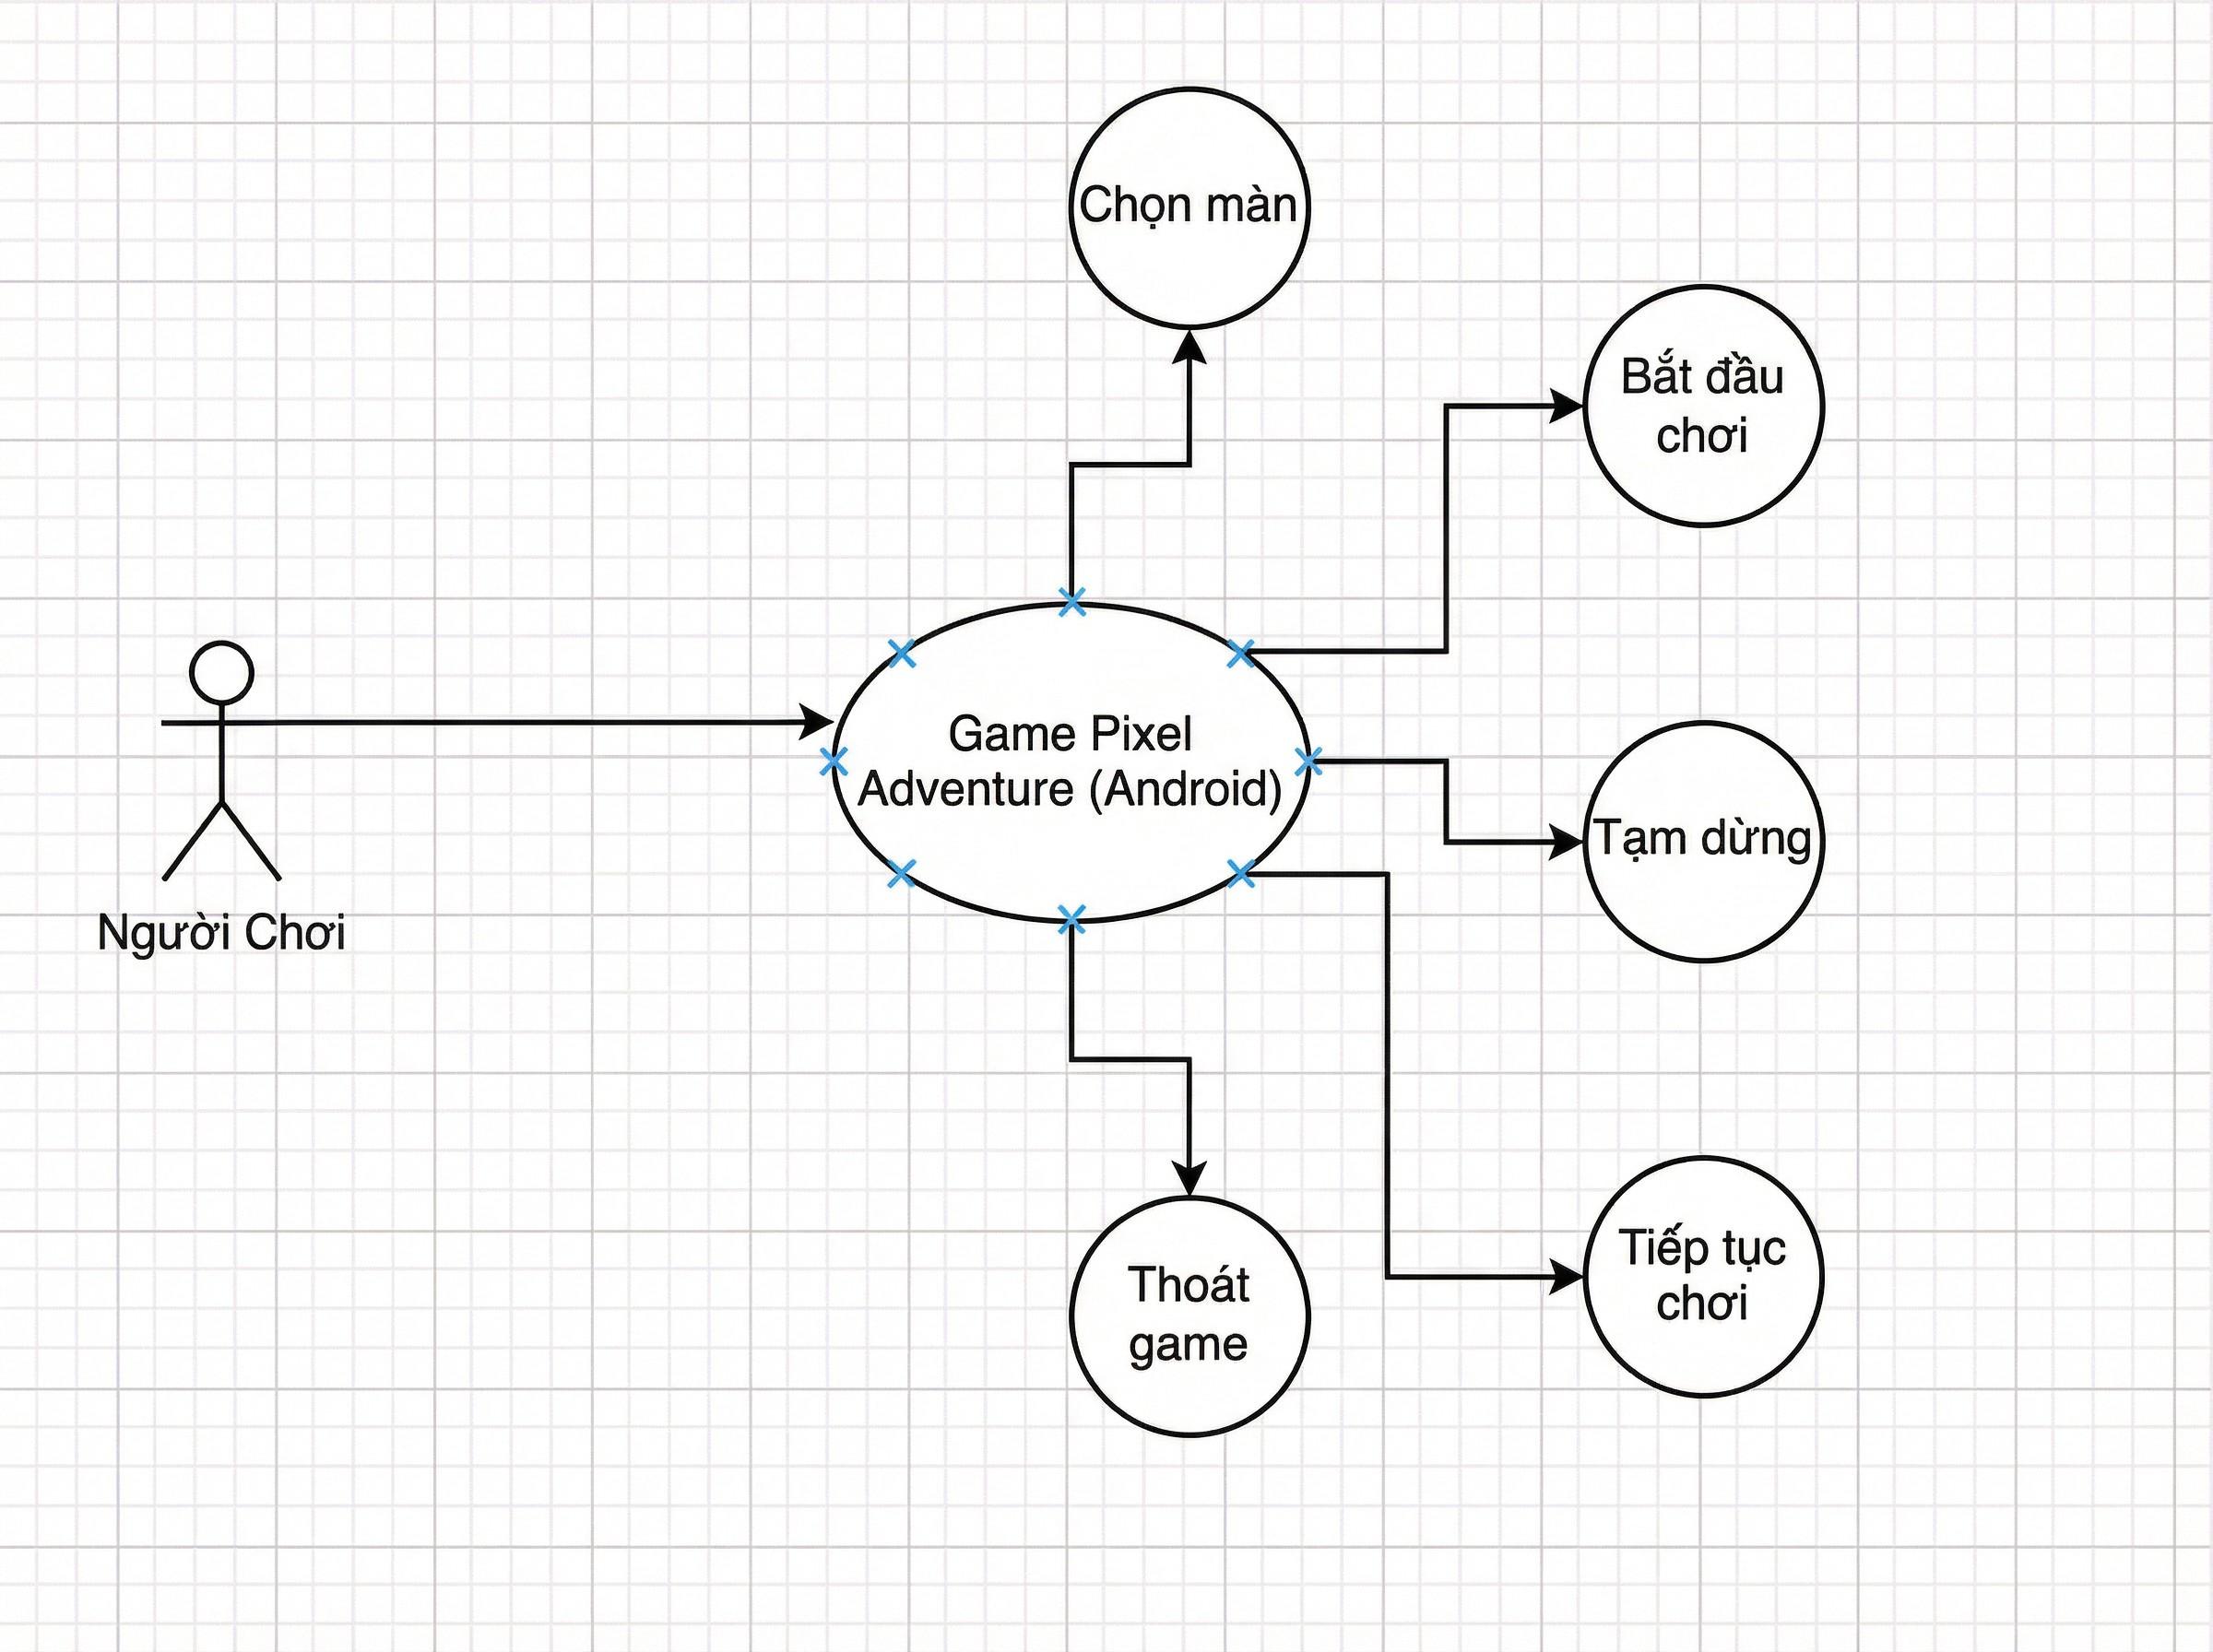
\includegraphics[width=9cm]{Đảo màu (5).jpeg}\\[3cm]
    \item Người chơi khởi động game, vào Menu chính.
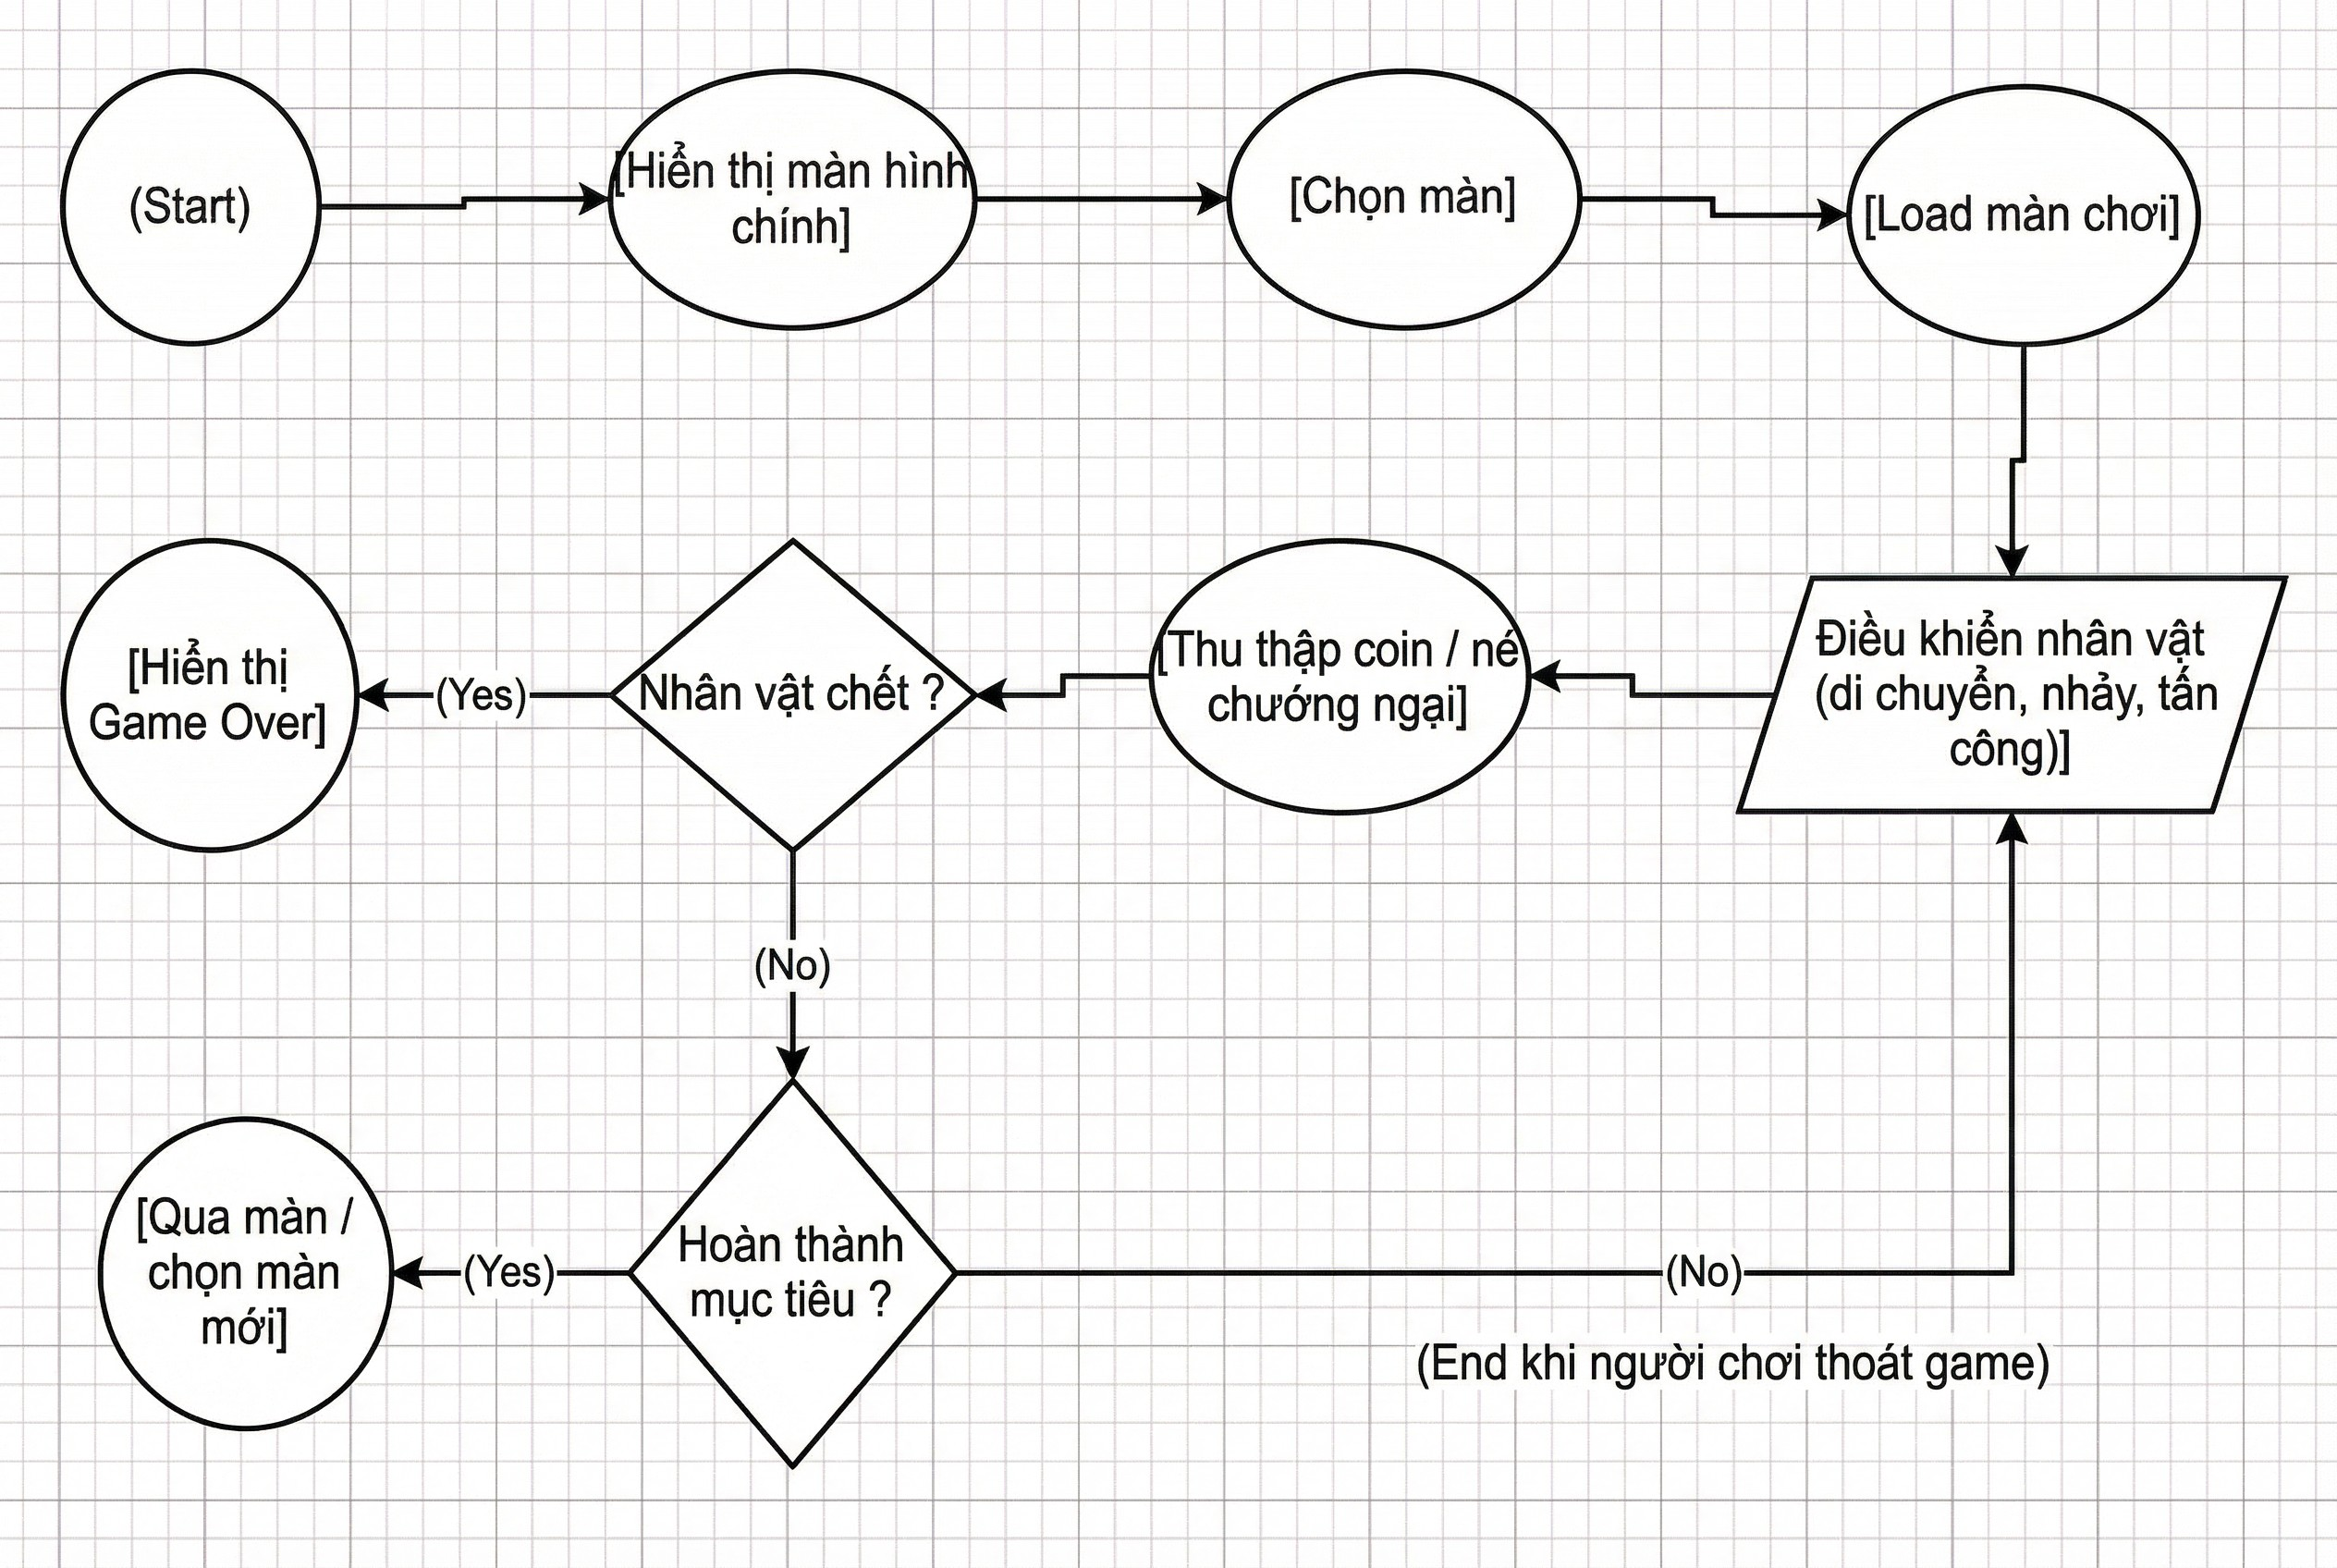
\includegraphics[width=9cm]{Đảo màu (4).jpeg}\\[3cm]
    \item Người chơi chọn level để chơi.
    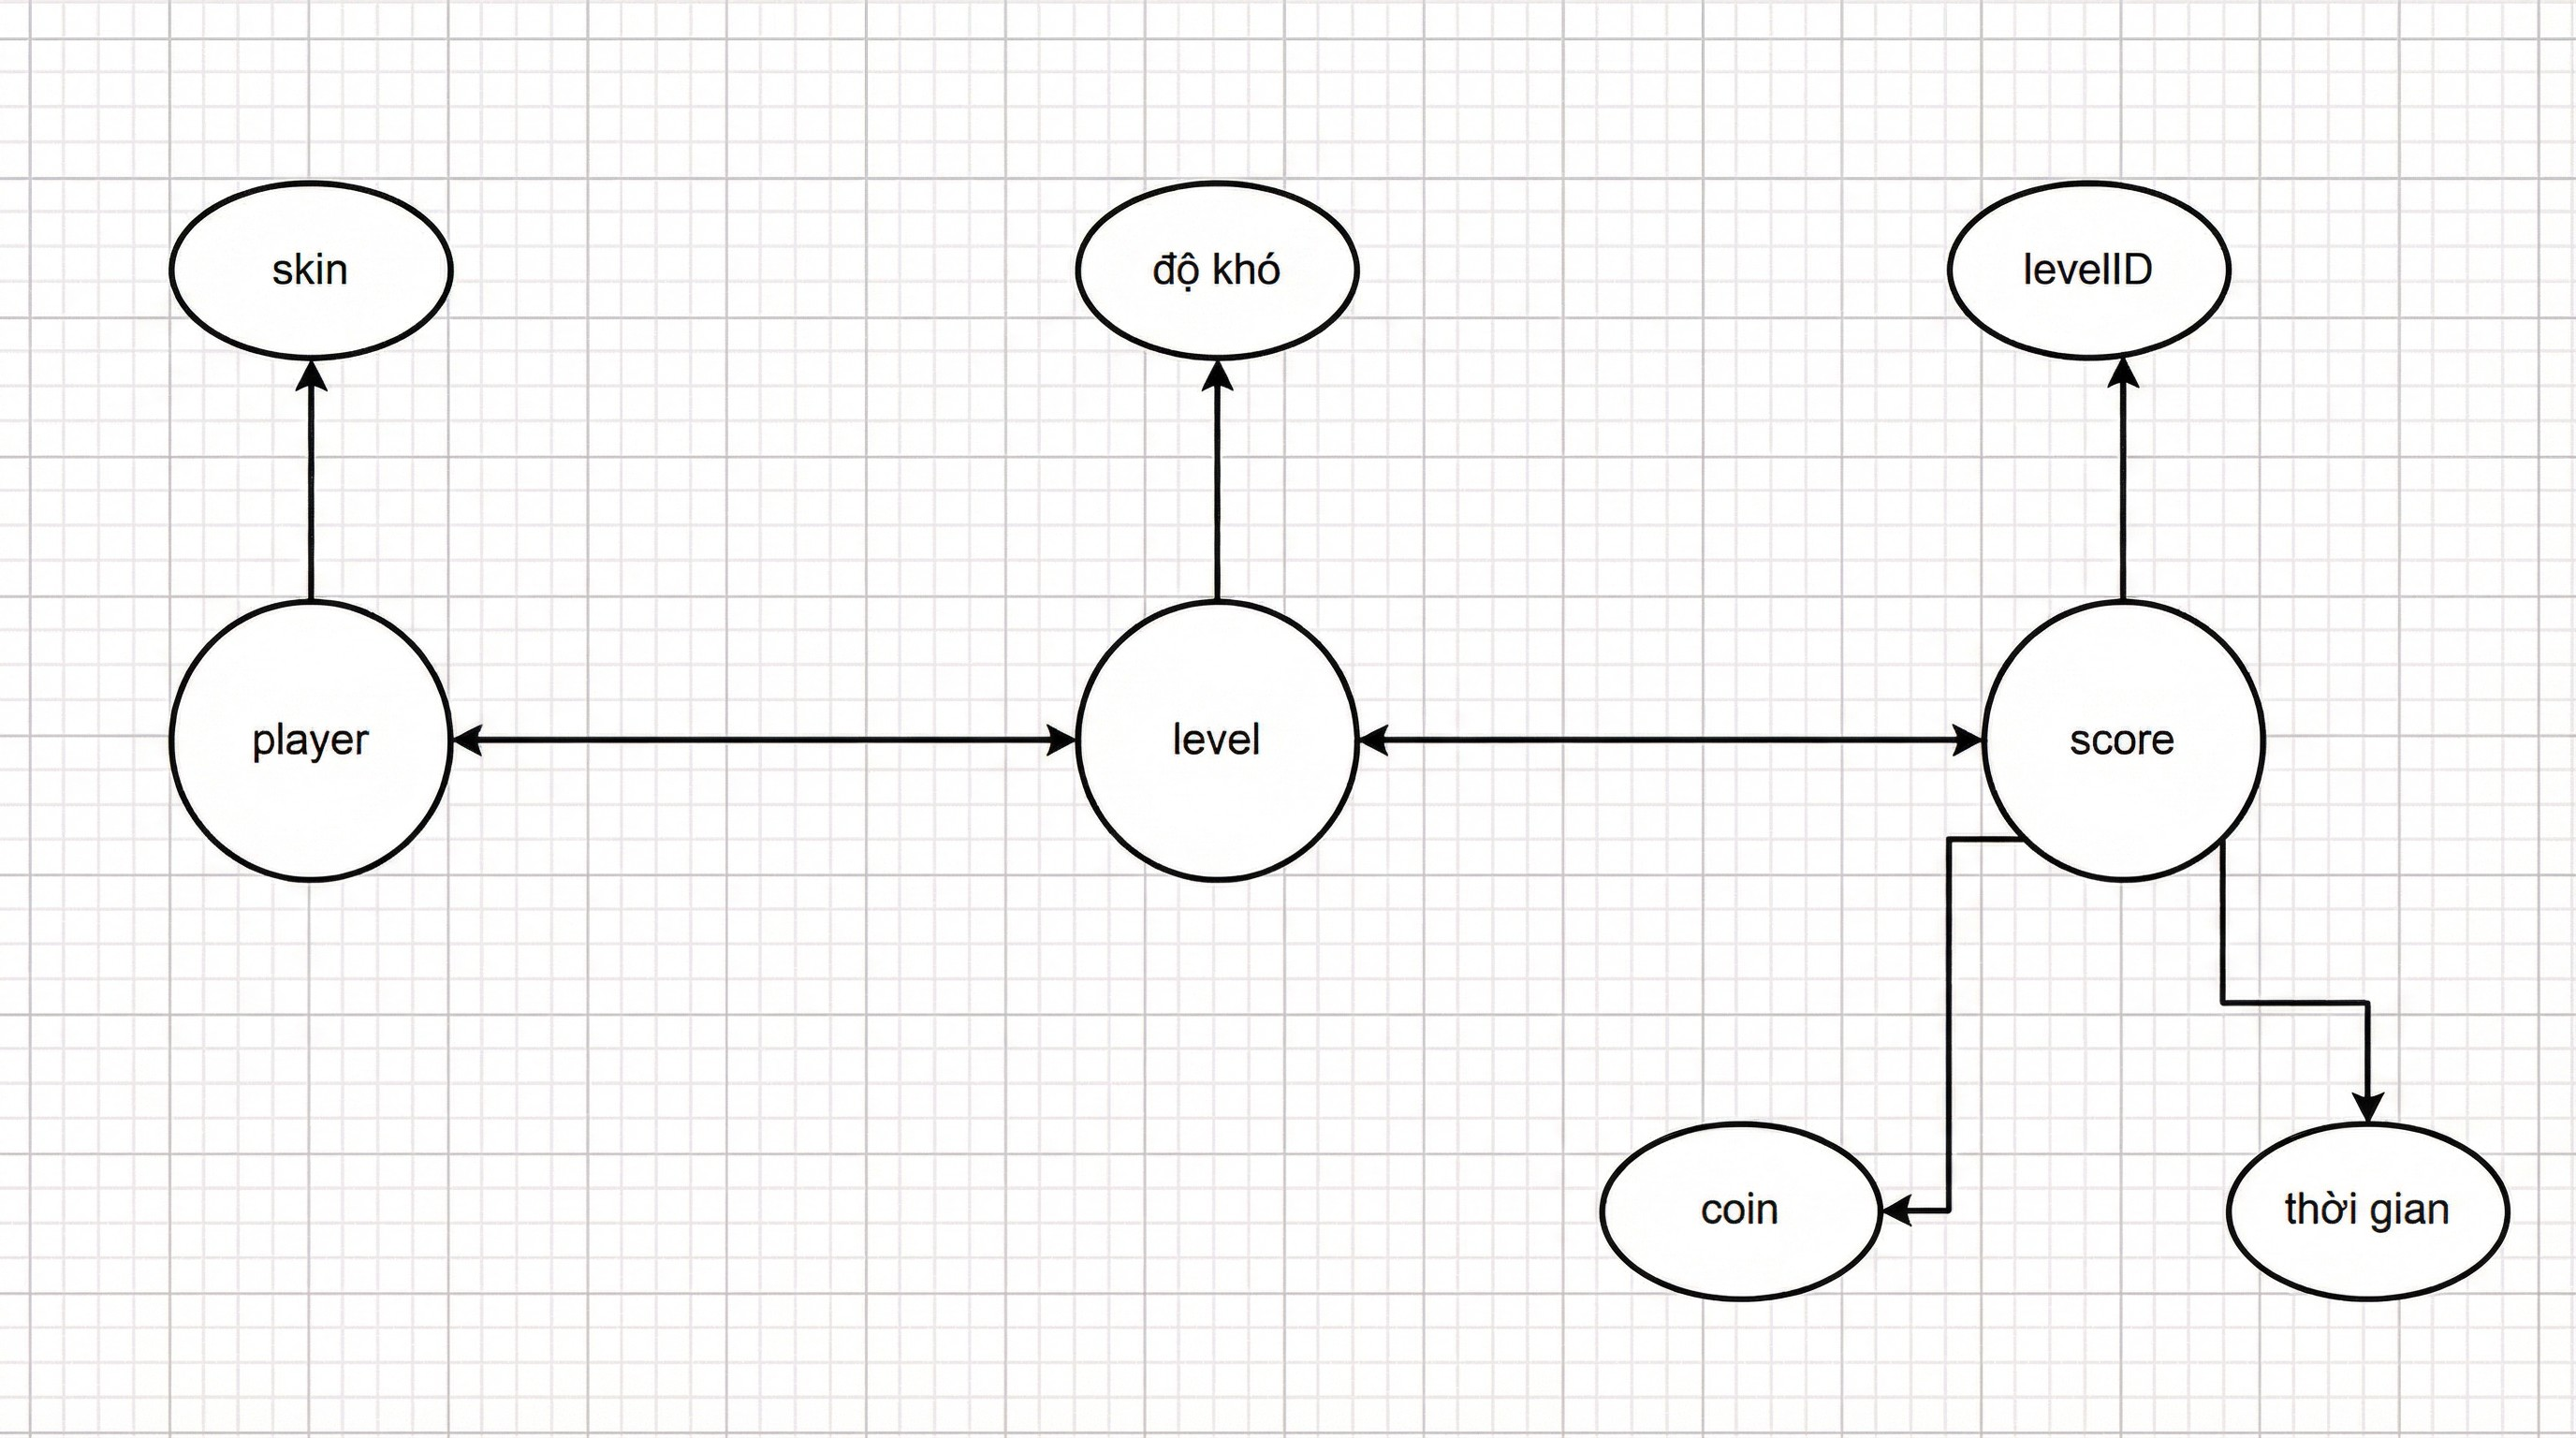
\includegraphics[width=9cm]{Đảo màu (1).jpeg}\\[3cm]
    \item Trong màn chơi: điều khiển nhân vật, thu thập coin, tránh bẫy, tiêu diệt kẻ địch.
    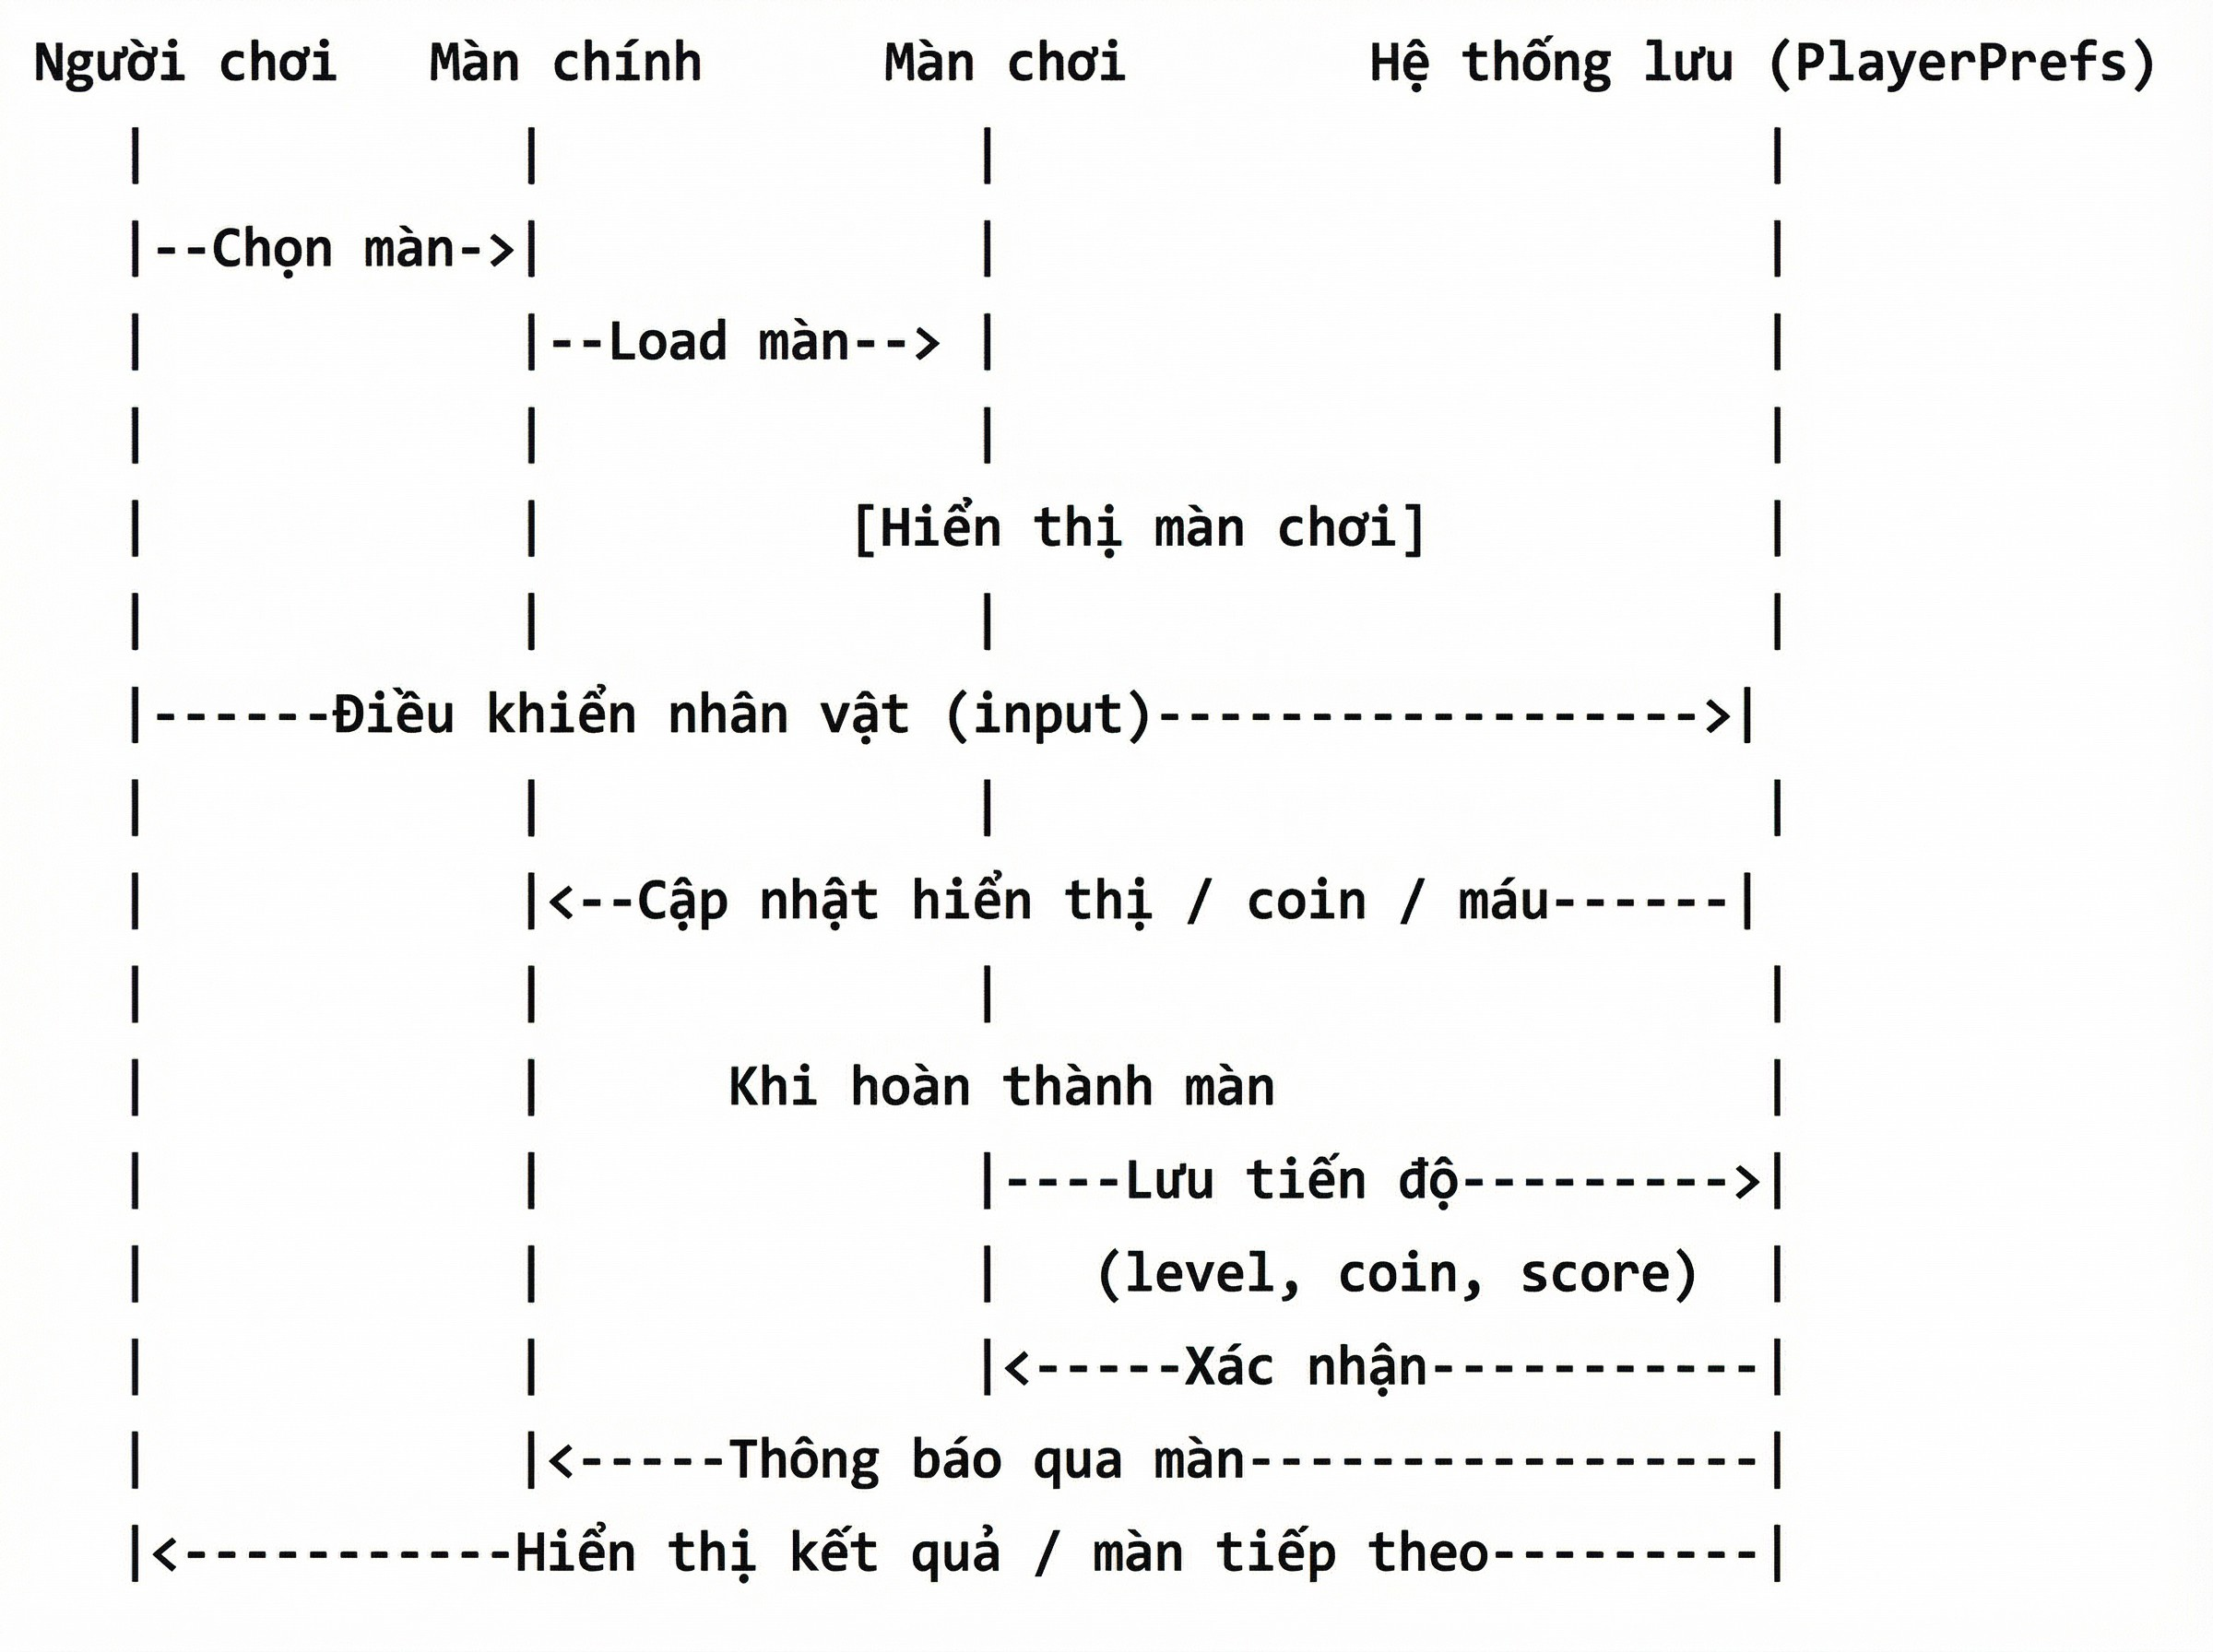
\includegraphics[width=9cm]{Đảo màu (3).jpeg}\\[3cm]
    \item Kết thúc màn chơi: Win hoặc Game Over, lựa chọn chơi lại hoặc quay về Menu.
    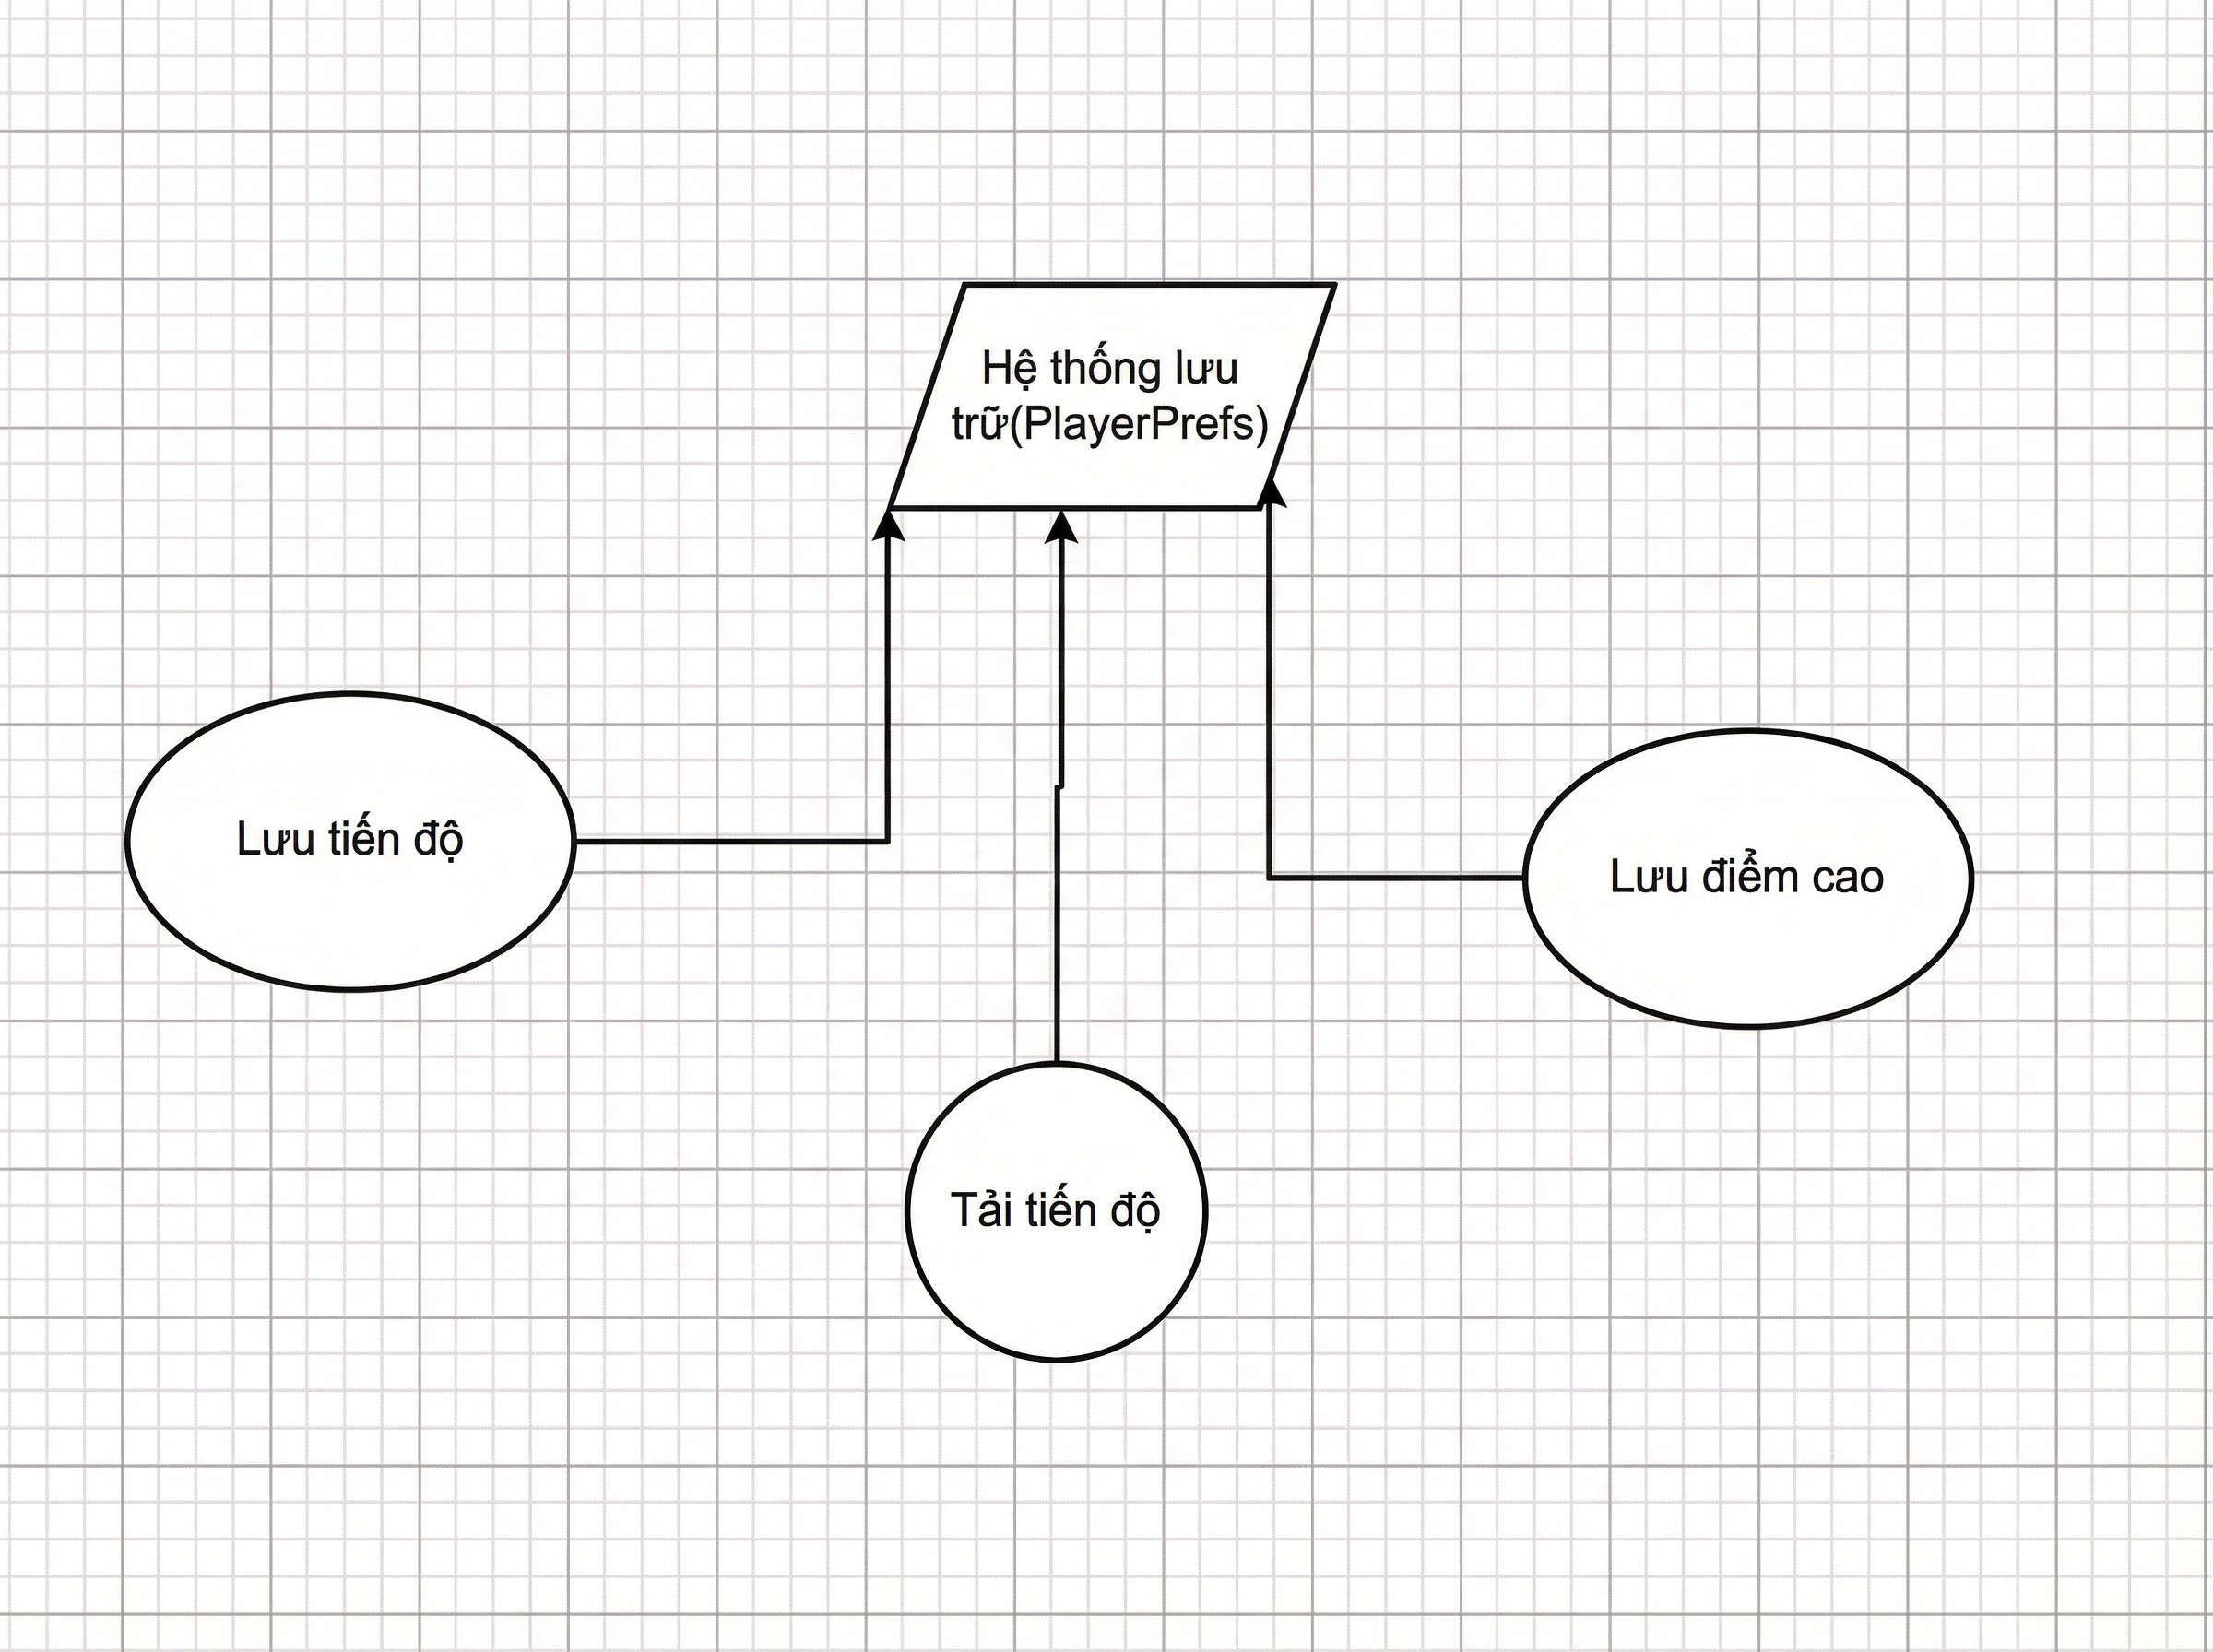
\includegraphics[width=9cm]{Đảo màu (2).jpeg}\\[3cm]
\end{itemize}
\subsection{Kiến trúc hệ thống}
Hệ thống được thiết kế theo mô hình component-based của Unity, gồm các module chính:
\begin{itemize}
    \item \textbf{Player}: Điều khiển nhân vật chính, xử lý input và va chạm.
    \item \textbf{Enemy}: Quản lý hành vi kẻ địch.
    \item \textbf{Item}: Vật phẩm, coin, power-up.
    \item \textbf{UI \& HUD}: Quản lý giao diện, score, timer, panel.
    \item \textbf{Level Management}: Quản lý chuyển cảnh, load level.
    \item \textbf{Sound Manager}: Quản lý nhạc nền và hiệu ứng âm thanh.
\end{itemize}

\newpage

% ================= CHƯƠNG 4 =================
\section{TRIỂN KHAI GAME}

\subsection{Giao diện và màn chơi (Scene -- UI -- HUD)}

Game bao gồm hai scene chính:
\begin{itemize}
    \item \textbf{Menu}: Giao diện chính, cho phép chọn nhân vật (nếu có), chọn level, bắt đầu chơi hoặc thoát game.
    
    \item \textbf{Game}: Màn chơi chính, nơi diễn ra toàn bộ hoạt động gameplay.
\end{itemize}

Trong quá trình chơi, HUD hiển thị:
\begin{itemize}
    \item \textbf{Score}: Điểm hiện tại dạng ba chữ số (ví dụ: 000, 010, 120).
    \item \textbf{Timer}: Thời gian chơi dạng MM:SS.
    \item \textbf{Các nút chức năng}: Pause, quay về Menu, chơi lại.
\end{itemize}

\subsection{Điều khiển nhân vật và tương tác}

\textbf{Cơ chế di chuyển:}
\begin{itemize}
    \item Di chuyển ngang sang trái/phải.
    \item Nhảy và hỗ trợ double-jump (nhảy hai lần nếu tính năng bật).
\end{itemize}

\textbf{Tương tác vật thể:}
\begin{itemize}
    \item Thu thập coin: Khi chạm vào, coin biến mất, phát âm thanh và tăng điểm.
    \item Va chạm với kẻ địch hoặc trap: Nếu va chạm từ bên cạnh hoặc từ dưới $\rightarrow$ Game Over.
    \item Stomp (nhảy lên đầu kẻ địch): Kẻ địch bị tiêu diệt, người chơi bật nảy và được cộng điểm.
\end{itemize}

\subsection{Kẻ địch -- vật cản -- vật phẩm}

\textbf{Kẻ địch:}
\begin{itemize}
    \item Tuần tra trong một vùng định sẵn, đổi hướng khi gặp mép vực hoặc chướng ngại.
    \item Bị tiêu diệt khi người chơi stomp từ trên xuống.
\end{itemize}

\textbf{Vật cản và bẫy:}
\begin{itemize}
    \item Các trap được bố trí tại những vị trí khó, buộc người chơi phải canh thời gian và quỹ đạo di chuyển hợp lý.
    \item Va chạm với trap sẽ dẫn đến Game Over.
\end{itemize}

\textbf{Vật phẩm:}
\begin{itemize}
    \item Coin là vật phẩm chính, dùng để tính điểm.
    \item Có thể mở rộng thêm các loại vật phẩm khác trong tương lai (tăng tốc, bảo vệ, \ldots).
\end{itemize}

\newpage

% ================= CHƯƠNG 5 =================
\section{KIỂM THỬ VÀ KẾT QUẢ}

\subsection{Kiểm thử gameplay}

\textbf{Mục tiêu:}
\begin{itemize}
    \item Đảm bảo các hành vi trong game hoạt động đúng như thiết kế: di chuyển, nhảy, thu coin, stomp, game over, win.
    \item Đảm bảo HUD cập nhật đúng, panel xuất hiện đúng thời điểm.
\end{itemize}

\textbf{Một số case kiểm thử tiêu biểu:}
\begin{itemize}
    \item Nhân vật di chuyển và nhảy mượt mà, không bị kẹt.
    \item Thu coin: mỗi coin chỉ thu được một lần và cộng đúng số điểm.
    \item Stomp kẻ địch: enemy bị tiêu diệt, score tăng, player bật nảy.
    \item Chạm trap hoặc enemy sai hướng: xuất hiện màn hình Game Over.
    \item Hoàn thành level: hiển thị màn hình Win, cho phép Next Level hoặc trở về Menu.
\end{itemize}

\subsection{Kiểm thử hiệu năng trên Android}

\textbf{Mục tiêu:}
\begin{itemize}
    \item Game chạy ổn định trên thiết bị Android phổ biến.
    \item FPS đạt mức chấp nhận được (từ 30 trở lên).
\end{itemize}

\textbf{Kết quả:}
\begin{itemize}
    \item Game chạy mượt trên các thiết bị tầm trung.
    \item Không xảy ra hiện tượng treo máy hoặc crash trong quá trình test.
\end{itemize}

\subsection{Lỗi gặp phải và cách khắc phục}

\begin{itemize}
    \item \textbf{Lỗi stomp không nhận đúng:} Điều chỉnh collider, thêm collider phần đầu enemy để dễ nhận stomp.
    \item \textbf{Lỗi UI không nhận input:} Kiểm tra lại thứ tự Canvas, Graphic Raycaster, và Event System.
    \item \textbf{Hiện tượng giật nhẹ khi có nhiều enemy:} Tối ưu lại số lượng enemy, sử dụng object pooling nếu cần.
\end{itemize}

\newpage

% ================= CHƯƠNG 6 =================
\section{ĐÁNH GIÁ VÀ HƯỚNG PHÁT TRIỂN}

\subsection{Ưu điểm}

\begin{itemize}
    \item Gameplay rõ ràng, dễ làm quen, phù hợp với game 2D platformer cơ bản.
    \item Giao diện đơn giản, thân thiện với người dùng, tối ưu cho màn hình ngang trên Android.
    \item Kiến trúc mã nguồn tách biệt theo từng thành phần (player, enemy, UI, \ldots), dễ bảo trì và mở rộng.
\end{itemize}

\subsection{Hạn chế}

\begin{itemize}
    \item Số lượng màn chơi còn ít, chưa tạo được chiều sâu về nội dung.
    \item Chưa tích hợp thêm các tính năng nâng cao như: hệ thống nhiệm vụ, lưu trữ cloud, bảng xếp hạng online.
    \item Hiệu năng ở một số thiết bị cấu hình thấp vẫn có thể cần tối ưu thêm.
\end{itemize}

\subsection{Định hướng phát triển}

\begin{itemize}
    \item Mở rộng thêm nhiều level, tăng dần độ khó và đa dạng kẻ địch, bẫy, môi trường.
    \item Bổ sung hệ thống vật phẩm đặc biệt (power-up), boss, kỹ năng nhân vật.
    \item Tích hợp lưu trữ dữ liệu, bảng xếp hạng và chia sẻ thành tích.
    \item Tối ưu hiệu năng hơn nữa, hướng đến phát hành trên Google Play.
\end{itemize}

\newpage

% ================= TÀI LIỆU THAM KHẢO =================
\section*{TÀI LIỆU THAM KHẢO}
\addcontentsline{toc}{section}{TÀI LIỆU THAM KHẢO}

\begin{enumerate}
    \item Unity Technologies, \textit{Unity Documentation – Hướng dẫn sử dụng Unity}, Tài liệu nội bộ, 2021.
    \item Unity Asset Store, \textit{Bộ sưu tập tài nguyên đồ họa Pixel Art và Asset cho Unity}, Nhà xuất bản Unity, 2022.
    \item Brackeys, \textit{Hướng dẫn lập trình Unity 2D Platformer}, Tài liệu học tập dành cho người phát triển game, 2020.
    \item Blackthornprod, \textit{Thiết kế Pixel Art và Game Design cho người mới bắt đầu}, NXB Game Dev Training, 2021.
    \item Ruben Ward, \textit{Kỹ thuật tối ưu hiệu suất game mobile bằng Unity}, NXB Mobile Game Tech, 2023.
    \item Microsoft Corporation, \textit{Lập trình C\# và Nguyên lý OOP trong phát triển game Unity}, NXB Công Nghệ Thông Tin, 2020.
    \item Kenney Studio, \textit{Tài nguyên Sprite Pixel Art phục vụ thiết kế game 2D}, NXB Creative Art, 2022.
    \item Chris Bradfield, \textit{Phát triển game 2D bằng Unity – Cơ bản đến nâng cao}, NXB Game Dev Guides, 2023.
\end{enumerate}

\end{document}
